\chapter{Selectivity of fengycin on phospholipids}
\label{c:chapter2}
\addcontentsline{toc}{chapter}{No selectivity towards model bacterial membrane}

\section{Outline}
\label{s:ch2_abstract}
Fengycin is a cyclic lipopeptide which is used as an
agricultural fungicide. It is synthesized by
\textit{Bacillus subtilis} as an immune response
against fungal infection, and functions by damaging
the target's cell membrane. Previous molecular dynamics
simulations and experiments led to the hypothesis that aggregation
of fengycins on the membrane surface plays a key role
in cell disruption. Here, we used microsecond scale
all-atom molecular dynamics simulation to understand
the specificity, selectivity, and structure of
fengycin oligomers. Our simulations suggest that
fengycin is more likely to form stable oligomers in
model fungal membranes (PC) compared to model
bacterial membranes (PE:PG). Furthermore, we
characterize differences in the structure and
kinetics of the membrane-bound aggregates and
discuss their functional implications.

\section{Introduction}
\label{s:ch2_intro}
Lipopeptides are a class of antibiotics which can effectively act against a
plethora of disease-causing organisms.\cite{Jacques2007} Many are
expressed by bacteria and can have both antibacterial and antifungal activity.
Fengycin, along with surfactins and iturins, is a member of a family of cyclic
lipopeptides originally obtained from \textit{Bacillus subtilis}. This bacteria
grows synergistically in the roots of leguminous plants where it protects them from
phytopathogens.\cite{Thonart2005} Fengycin acts as a fungicide and can be used
to treat various diseases in plants like clubroot disease (\textit{Plasmodiophora monoliforme}),
maize rot (\textit{Fusarium moniliforme}), barley
head blight (\textit{Fusarium graminearum}), and cucurbit powdery (\textit{Podosphaera fusca}).
\cite{Jung1986,Long2013,Yang2007,Chan2009,RomeroPerez2007} Biocontrol agents
like fengycin avoid the adverse effects of chemical pesticides and are
eco-friendly. Through genetic modifications, certain strains of \textit{B.
subtilis} are capable of over-producing lipopeptides, which led to the
development of the commercially available biofungicide
Serenade\textsuperscript{TM}(Bayer).

There are two methods by which fengycin acts against these fungi. First, it
induces systemic resistance in the plants by perturbing the cell membrane of
the root cells.\cite{Jacques2007,Thonart2007} Second, fengycin directly attacks
fungi by binding to their cell membrane, causing leakage and
lysis.\cite{Seelig2007,Heerklotz2011,Nylander2008,Nylander2005} In this work, we
will focus on the latter phenomenon.

Beyond its established agricultural applications, fengycin (and related
compounds) show promise as antifungal drugs. Fengycin has low hemolytic
activity, and the combination of D-amino acids and cyclic structure makes it
less vulnerable to degradation by peptidases compared to conventional antimicrobial peptides.
\cite{Jung1986} Furthermore, membrane composition varies slowly in an evolutionary sense,
slowing the advent of fungal resistance. In addition, fengycin has been found to be effective
against filamentous fungi and hypothesized to be effective against
localized dermatomycosis.\cite{Dufrene2005,Deleu2013} After the approval of daptomycin,
present in the drug Cubicin, increasing efforts to find lipopeptide-based drugs
have increased.\cite{Kirkpatrick2003} Thus, understanding how fengycin interacts with bilayers will
help us understand how best to use it as a basis for future drug development.

Coarse-grained MD simulations of individual and oligomerized fengycins in
various lipid bilayers suggest that they bind to all membranes with their acyl
chains inserted into the hydrophobic core.\cite{HornGrossfield2013} These
simulations also showed that membrane composition affected fengycin's tendency
to aggregate in the membrane; specifically, the aggregates are stable in
bilayers made with phosphatidylcholine (PC) headgroups (typical of eukaryotic
cells), but not in bacterium-like mixtures of phosphatidylethanolamine (PE) and
phosphatidylglycerol (PG). The authors hypothesized that the aggregates, which
significantly bend and distort the membrane, are the active form of the
lipopeptide.
These results were highly suggestive, but the limitations of a coarse-grained force field in
representing detailed packing and electrostatic interactions require they be
confirmed by all-atom simulations, particularly given the number of charged moieties in the system.

The goal of the present work is to clarify the composition-specific
effects of fengycin on model lipid bilayers chosen to mimic eukaryotic
and bacterial membranes via all-atom molecular dynamics simulations.
The simulations demonstrate statistically significant differences
between the lipopeptides' behavior depending on the nature of the
lipid headgroups, with resulting differences in their effects on bilayer structure.

\section{Methods}
\label{s:ch2_methods}

\subsection{Chemical Structure of fengycin} 
\label{ss:ch2_chem_str} 

\begin{figure}
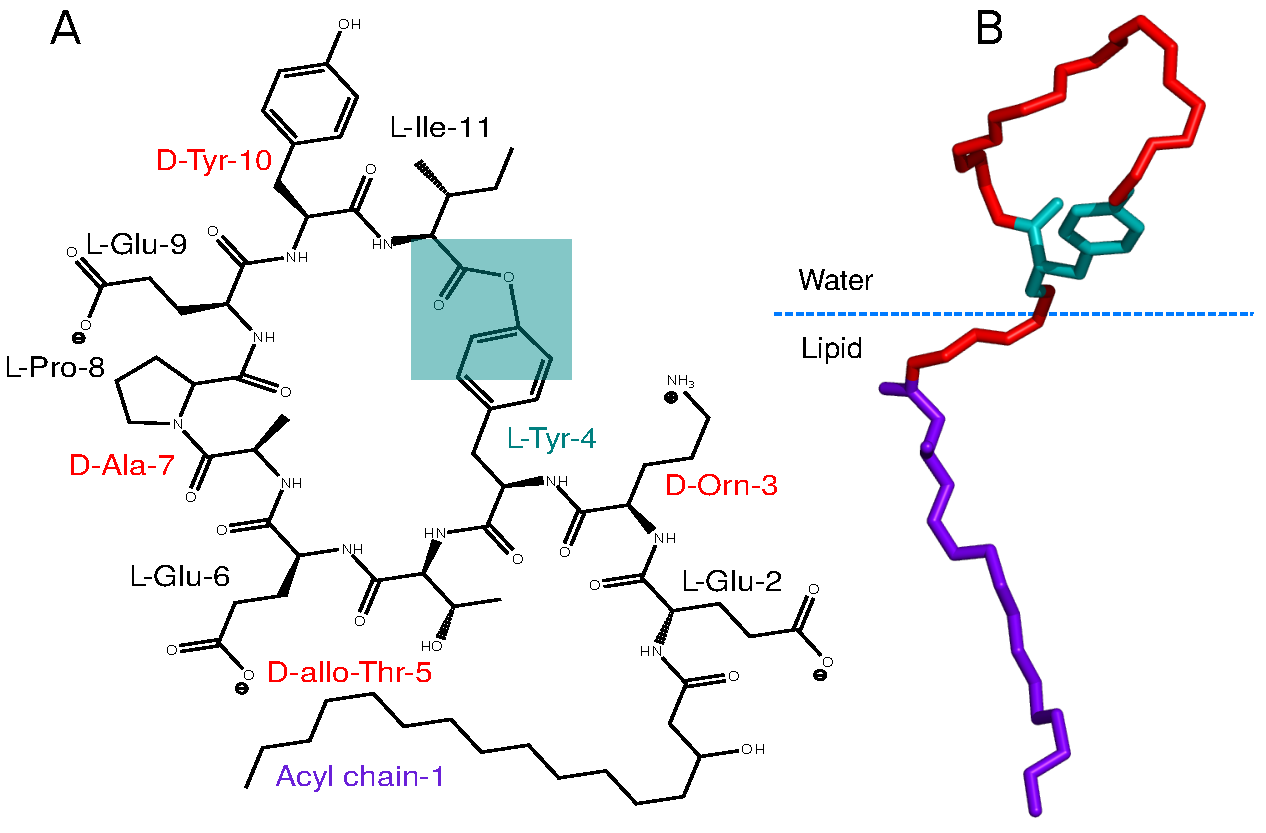
\includegraphics[width=0.58\textwidth]{chapter2_figs/structure.pdf}
\caption{\label{fig:ch2_chemical_str} (A) Chemical
structure of fengycin(Adapted from Horn et al).\cite{Liu2007,HornGrossfield2013};
 (B) 3D orientation of one of the
conformations of fengycin during our simulation.
Violet sticks represent the acyl tail, red sticks
show the peptide backbone and cyan sticks stand for
the C-terminus and Tyr-4 ester linkage.}
\end{figure}

Fengycin is an
amphipathic cyclic lipopeptide, with the chemical structure shown in \textbf{Figure
\ref{fig:ch2_chemical_str}}. It consists of an anionic cyclic decapeptide with a
$\beta \mbox{-}$hydroxy fatty acid attached at the N-terminus.
\cite{HornGrossfield2013} Fengycin naturally occurs with a number of variations in the protein sequence and acyl
chain length; the specific fengycin used in the present simulations was first
reported by Wu et al and characterized by Pathak et al using mass spectroscopic
techniques.\cite{Liu2007,Balaram2012} This particular variant has several
distinctive features: (i) four D-amino acid residues
(tyrosine (Tyr-10) , alanine (Ala-7), non-natural ornithine (Orn-3) and threonine (Thr-5));
(ii) three negatively charged glutamate (Glu-2, Glu-6, Glu-9) residues; and one positively charged
residue Orn-3, resulting in a net charge of -2; (iii) cyclic structure with the
ring closure occurring between Tyr-4 and Ile-11 through an ester bond.



\subsection{System Construction} 
\label{ss:ch2_sys_constr} 
Fengycin has some unusual
moieties not found in the standard CHARMM36 forcefield, including the $\beta \mbox{-}$hydroxyl
on the acyl chain and the ester bond connecting the C-terminus to
Tyr-4. Parameters for these atoms were developed using the Forcefield
toolkit (FFTK) plugin to VMD \cite{Gumbart2013,Schulten1996}. A stream file (feng\_stream.txt)
containing all new parameters is attached as supplemental information.
The lipopeptide structures were built using a modeling tool, Molefacture
 which is found as an extension of VMD.\cite{Schulten1996}

We constructed a membrane-bound fengycin system by placing molecules randomly on
two planes parallel to the z-axis with the acyl chains pointed towards the
membrane center, producing systems with 10 lipopeptides in each leaflet. The
choice to run symmetric systems is an attempt to model the long-time equilibrium
behavior accessible to experiments such as the fluorescence work from Heerklotz
and coworkers \cite{Heerklotz2011}. However, this choice does mean that membrane
deformations due to asymmetric binding are not accessible; some antimicrobial
peptides seem to exploit that asymmetry to induce pores, with the result that at
long times their activity goes away due to peptide migration to the inner
leaflet \cite{Wimley2012}.

The Optimal Membrane Generator (OMG) package from LOOS was used to place lipids
around fengycin and solvated the system.\cite{Grossfield2009,Grossfield2015} The
system was electronically neutralized with excess sodium ions, with additional
NaCl added to bring the free salt concentration to appromixately 100mM. We
modeled water using TIP3P, as is appropriate with the CHARMM forcefield. The
system was thoroughly minimized and equilibrated through a series of alternating
minimizations and short dynamics runs.

Table 1 summarizes the different systems run. To model the gram-negative
bacteria we used a 2:1 mixture of palmitoyl-oleoyl-phosphatidylethanolamine (PE)
and palmitoyl-oleoyl-phosphatidylglycerol (PG). A pure palmitoyl-oleoyl-phosphatidylcholine
(PC) bilayer was used to emulate a eukaryotic membrane. The
lipopeptide-lipid systems had 10 fengycins bound to each leaflet of the lipid
bilayer. As a control, we ran simulations of neat bilayers with the same
compositions. For each lipopeptide system, we ran 4 independently constructed
replicates, while for the pure lipid systems we ran 3 replicates of each. All
the systems have 90 lipids per leaflet.

\begin{table}
  \caption{Summary of simulations}
  \label{tbl:ch2_sys_cons}
  \begin{tabular}{llccc}
    \hline
    \textbf{System}  & \textbf{Phospholipids} & \textbf{fengycins per leaflet} & \textbf{Length(ns)} & \textbf{\# of replicates} \\
    Bacteria   & PE:PG & 10 & $\sim$5000  & 4 \\
    Fungus & PC  & 10 & $\sim$4500 & 4\\
    Neat  & PE:PG & 0 & $\sim$150 & 3\\
    Neat & PC & 0 & $\sim$150 &3\\
    \hline
  \end{tabular}
\end{table}

\subsection{Simulation protocol}
\label{ss:ch2_sim_proto}

All simulations were run with NAMD version 2.9 \cite{Schulten2005}. We used the
CHARMM36 forcefield for both the peptide and lipid, including the CMAP
correction for the peptide backbone; the D-amino acids were
represented by defining a new atom type for the D-$\alpha$ carbon and
transposing the matrices for the CMAP values (see the parameters for D-Orn in
the supplemental information).\cite{Grossfield2013,MacKerell2013,Pastor2010}

We used Langevin dynamics for all heavy atoms with the temperature set to
310.5K, and the Langevin piston barostat, with semi-isotropic
boundary conditions.\cite{Stoll1978,Brooks1995,Klein1994} We used smooth particle-mesh Ewald summation with a
96x96x96 grid to calculate long-range electrostatics.\cite{Ewald1921} Van der Waals interactions
were smoothly cutoff from 8 to 12 {\AA} with the pairlist maintained at 14 {\AA}.
We used a 2 fs timestep with the bonds constrained to their equilibrium lengths
using the RATTLE algorithm.\cite{Andersen1983}

\subsection{Simulation Analysis}
\label{ss:ch2_sim_ana}

All analyses were done at 1 ns resolution unless otherwise specified.  For
equilibration purposes, we excluded the first 500 ns of the lipopeptide
simulations and 100 ns of the pure membrane simulation. All
analysis was performed with tools developed using LOOS, a software package for the analysis of molecular dynamics simulations,
 available for download from https://github.com/GrossfieldLab/loos.\cite{Grossfield2014,Grossfield2009}
Unless otherwise noted, all error bars are standard errors in the mean, computed by treating each trajectory as an individual measurement.

\subsubsection{Radial Distribution Functions}
\label{sss:ch2_rdf}
We determined the three-dimensional radial distribution functions for various pairs of atoms using the
atomic\_rdf tool from LOOS.\cite{Grossfield2014,Grossfield2009} We also
calculated the radial distribution function in the membrane plane for fengycin
and the different lipid species using the xy\_rdf tool, also a part of LOOS; this tool operates on the molecules' centers of mass, rather
than individual atoms. The time evolution of these RDFs was also calculated by
dividing the trajectory into 10 ns windows and the resulting figure can be found in the \textbf{Supplemental Information}.

\subsubsection{Quantifying Aggregation}
\label{sss:ch2_agg}
We considered two lipopeptide molecules to be in contact if there were
at least ten pairs of heavy atoms within 3 {\AA} of each other.
Using this criterion, we calculated the number of lipopeptides in each aggregate
and determined the probability distribution of aggregate size.
We normalized the distribution by calculating the fraction of lipopeptides that are present in different
aggregate size.

\subsubsection{Residue-Residue Contact Map}
\label{sss:ch2_res-res_contact}

We quantify lipopeptide-lipopeptide interactions using residue contact maps.
The definition of a contact is similar to that described above: two residues are
in contact if they share at least ten pairs of heavy atoms within 3 {\AA}.
Fractional contacts are defined as the probability of a specific residue-residue
pair being in contact given that the two molecules are in contact.

\subsubsection{Lifetime of the aggregates}
\label{sss:ch2_lifetime}

In order to characterize the kinetic stability of differently sized aggregates,
we created a time series for each trajectory, assigning each frame a value of 1
 when a particular aggregate was present, and 0 if it was not.
We then calculated the autocorrelation function
for each such time series and averaged the resulting correlation
functions as a function of aggregate size.

\subsubsection{Order parameters}
\label{sss:ch2_ord_param}

To quantitate the effects of fengycin on lipid chain structure, we computed
order parameters analogous to those measurable via solid-state deuterium quadrupolar
splitting experiments. The order parameters are calculated using the second
Legendre polynomial applied to the angle $\theta$ between a
given acyl carbon-hydrogen bond and the membrane normal:

\begin{equation}
\label{eq:ch2_ord_par}
S_{CD} = \bigg |\left\langle \frac{1}{2} \left( 3 \cos^2 \theta - 1 \right)\right\rangle \bigg |
\end{equation}

This calculation was performed using the order\_params tool from LOOS. \cite{Grossfield2014,Grossfield2009}

\subsubsection{Molecular order parameters}
\label{sss:ch2_dibmop}

To characterize the length scale on which fengycin alters lipid chain structure,
we calculated the molecular order parameters for lipid chains as a function of
distance to the nearest fengycin, using the LOOS tool dibmops.\cite{Grossfield2014,Grossfield2009}
Analogous to the deuterium order parameter shown in \textbf{Eq. \ref{eq:ch2_ord_par}},
the molecular order parameter is the second Legendre polynomial of the angle between the membrane normal
and the average of the second and third principal axes of the chain.

\section{Results and Discussion}

\section{Results and Discussion}
  
\label{s:ch2_results}
\subsection{Fengycin causes disorder in membrane}

\label{subsec:ch2_opara}

One of the most common effects of antimicrobial peptides is reducing the order
of the surrounding lipids.\cite{Seelig2004} To quantify this, we computed order parameter
profiles for the lipid palmitoyl chains, as described in section \textbf{
\nameref{sss:ch2_ord_param}} under \textbf{\nameref{s:ch2_methods}}, with results shown in \textbf{Figure \ref{fig:ch2_ord_par}}.  As expected,
fengycin reduces the order parameters for all carbons between C-3 and C-15 relative
to their equivalents in neat membranes. This indicates an overall disordering effect
but does not indicate the length-scale on which fengycin operates.
To determine this, we computed the chain order parameter as a function of
distance, as discussed in section \textbf{\nameref{sss:ch2_dibmop}} under \textbf{\nameref{s:ch2_methods}}.
 \textbf{Figure \ref{fig:ch2_dibmop}} also shows that the molecular order parameter for membrane bilayers containing
fengycins are lower than the equivalent neat membranes, consistent with \textbf{Figure
\ref{fig:ch2_ord_par}}.  However, the effect is most pronounced for lipids within 10
{\AA} of the nearest fengycin, plateauing at longer range. In addition, the order
parameter remains lower than the neat membrane even at a very long range;
presumably, more distant lipids are altered by their disordered neighbors and
not by fengycin directly.

\begin{figure}
\centering
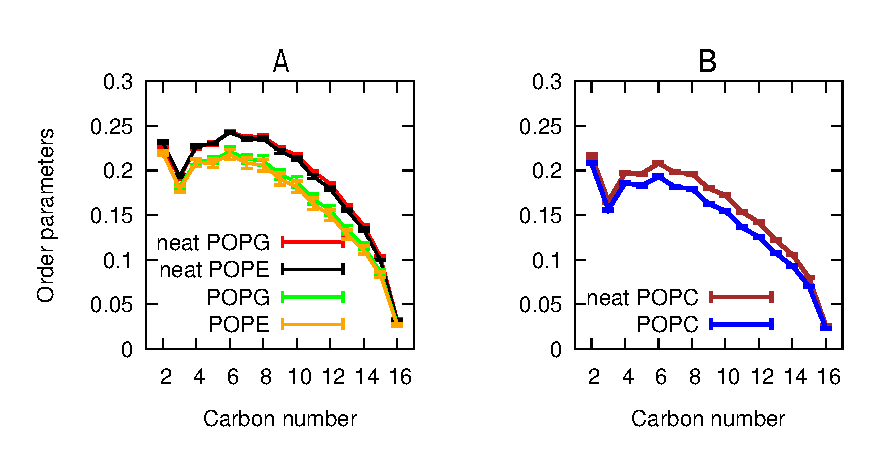
\includegraphics[width=0.7\textwidth]{chapter2_figs/ord_par_corr.pdf}
\caption{\label{fig:ch2_ord_par} Order parameters for the palmitoyl chain of
(A)PE:PG and (B)PC. Neat indicates order parameters for membrane systems without
any fengycin in them. The error bars indicate the standard error for each
replicate. Carbon number for the palmitoyl chain is along the x-axis while
average order parameter is along the y-axis.}
\end{figure}

\begin{figure}
\centering
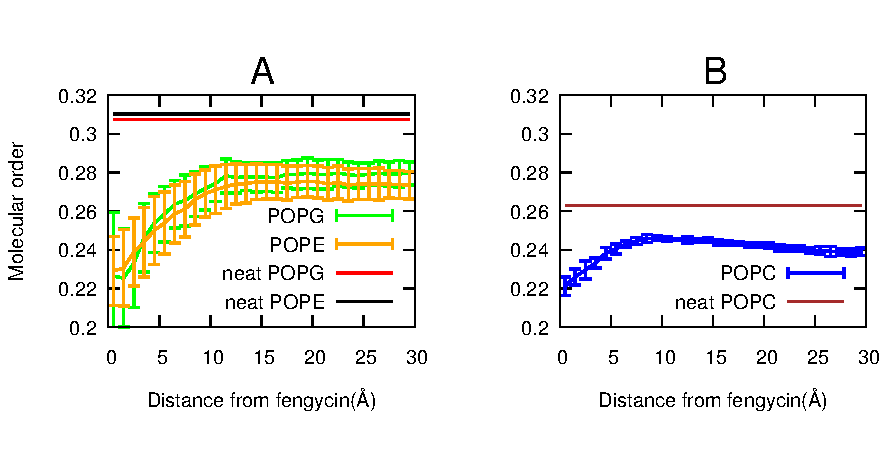
\includegraphics[width=0.7\textwidth]{chapter2_figs/dibmop_corr.pdf}
\caption{\label{fig:ch2_dibmop}Molecular order parameters of palmitoyl chain as a
function of distance from fengycin molecule.(A) is for PE:PG and (B) is for PC.
The error bars are the standard error for each replicate. Neat membranes (no
fengycins) are represented as straight lines.}
\end{figure}


\subsection{Preferential interaction with PE}
\label{subsec:xyrdf_feng_lipid}

In addition to altering the lipid chain structure, antimicrobial peptides can
also alter the lateral ordering of lipid headgroups .\cite{Epand2012,Epand2009}
 This is most easily quantified using a lateral
radial distribution function, as shown in \textbf{Figure \ref{fig:ch2_xyrdf_mem}}. Using the method described in \textbf{\nameref{sss:ch2_rdf}}
we calculated the radial distribution function between the center of masses of fengycin and different lipid types (PE,PG,PC).
\textbf{Figure \ref{fig:ch2_xyrdf_mem}A} shows that PE is significantly enriched in the first solvation shell surrounding fengycin,
while PG is equivalently depleted. By contrast, PC shows no evidence of structuring
around fengycin, other than steric depletion at short range.

The apparent attraction between fengycin and PE is likely due to two factors.
First, the PE amine group is a hydrogen bond donor, unlike the choline group in
PC, so it can make favorable interactions with the peptide's anionic side
chains.
Second, electrostatic repulsion between the peptide and PG, both of
which are negatively charged, could create an apparent attraction to the zwitterionic PE headgroup.

\begin{figure}
\centering
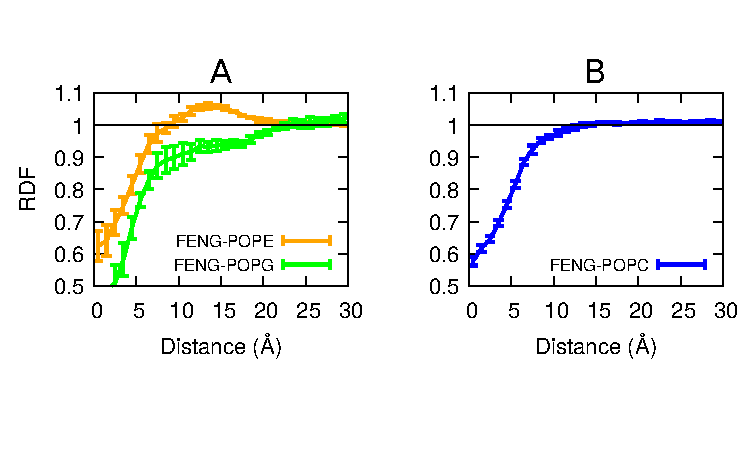
\includegraphics[width=0.7\textwidth]{chapter2_figs/feng_mem_corr.pdf}
\caption{\label{fig:ch2_xyrdf_mem} Radial distribution function in the membrane plane between
fengycin peptide ring and the lipid head group. (A) is for PE:PG and (B) is for PC.
Distance between the two sets of entities
is along the x-axis, while RDF is along the y-axis.
The straight line at 1 represents the RDF value for a
random distribution such as the ideal gas. The error bars are the standard error, treating each trajectory as a single measurement.
}
\end{figure}

\subsection{Headgroups attract charged fengycin residues}
\label{subsec:atomicrdf}
In order to test whether there are specific interactions that attract fengycin
to PE headgroups, we computed a series of three-dimensional radial distribution
functions as shown in \textbf{Figure \ref{fig:ch2_atomic_rdf}}.
 Please note that these values are inflated by the molecules' restriction to the membrane surface.
 We calculated the distribution of following specific atoms ---
(i)nitrogens of PE amines around oxygens in the carboxylate part of glutamates,
(ii)oxygens of the hydroxyl group in PG glycerols around nitrogen of amine in Orn-3
(iii)phosphates of PG and PC around nitrogen of amines in Orn-3.
These atoms were selected because they indicate most likely electrostatic attractions among themselves.
\textbf{Figure \ref{fig:ch2_atomic_rdf}} indicates that the phosphates and
hydroxyls in the lipid headgroups attract the positively charged ornithine side
chains, while the three negatively charged glutamates preferentially interact
with the positively charged amine of PE or with water. We do not see a net
attraction between fengycin and PG because the peptide has three glutamates but only
one ornithine.

Qualitatively, all the glutamates show similar preference patterns, but
quantitatively they are quite different. Glu-2 has a much higher contact peak with the PE amine,
indicating it spends more time in contact
than the other two glutamates. This difference is likely
due to the covalent structure of fengycin; Glu-2 is immediately adjacent
to the lipopeptide fatty acid, forcing the sidechain to remain at the
membrane-water interface.  By contrast, the other two glutamates are
part of the ring and can either be hydrated or interact with
lipid. The lateral ordering we observed for PE:PG section (\textbf{\nameref{subsec:xyrdf_feng_lipid}}) can be rationalized by the glutamates'
preferential packing with the PE amines.

Although PC phosphates can interact favorably with ornithine (see the upper
left panel of \textbf{Figure \ref{fig:ch2_atomic_rdf}}), overall  the electrostatic forces
are insufficient to create a net attraction between the peptide and PC
headgroups (see \textbf{Figure \ref{fig:ch2_xyrdf_mem}}).

\begin{figure}
\centering
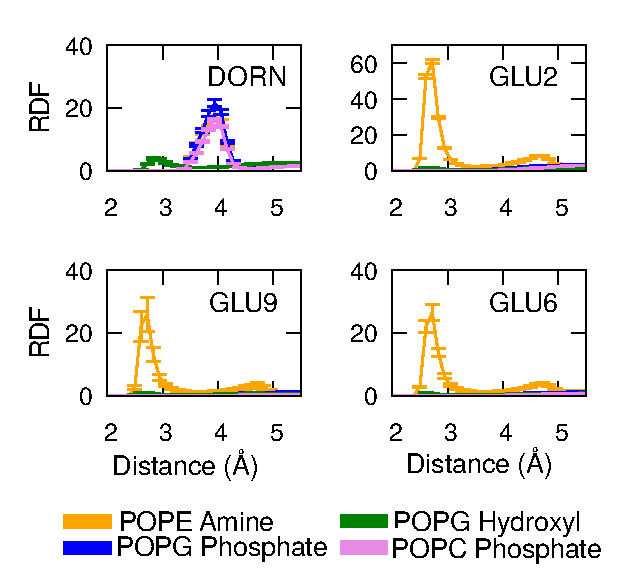
\includegraphics[width=0.7\textwidth]{chapter2_figs/atomic_rdf.pdf}
\caption{\label{fig:ch2_atomic_rdf} Three-dimensional radial distribution function between
charged atoms of D-ornithine (DORN) and Glutamates (GLU) in fengycin and head groups of
PE, PG and PC. RDF is along the y-axis and distance between the atoms is along the x-axis.
Note the upper right panel is plotted on a different y-scale.}
\end{figure}
\newpage

\subsection{Fengycin aggregation depends on membrane composition}
\label{subsec:fengxyrdf}
Our working hypothesis in performing these simulations was that the ability of
fengycin to damage target membranes was related to its aggregation.\cite{HornGrossfield2013}
 This in turn suggests that aggregation should vary with the bilayer's
lipid composition, so that fungal (eurkaryotic) membranes are damaged while the
native bacterial membranes are not.  To test this hypothesis, we first computed
the fengycin-fengycin lateral radial distribution function, shown in \textbf{Figure \ref{fig:ch2_feng_feng}}.

The fengycin-fengycin RDF in PC shows a single large peak at roughly 10 {\AA},
indicating significant peptide-peptide attraction and the presence of some
aggregates. Visual inspection of the trajectories confirms that aggregates
begin to appear after the first 500 ns to 1 $\mu$s. By contrast, the first peak
is significantly smaller in PE:PG membrane, but there is a small secondary peak
around 20 {\AA.} This indicates that while there is less aggregation overall in
the ``bacterial membrane'', there is a small tendency to form more elongated
structures.

\begin{figure}
\centering
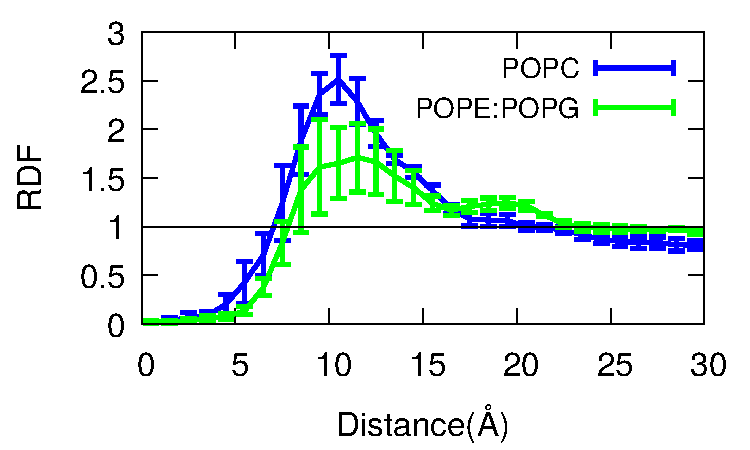
\includegraphics[width=0.4\textwidth]{chapter2_figs/feng_feng.pdf}
\caption{\label{fig:ch2_feng_feng} Lateral radial distribution function between
fengycins. Lipopeptide separation is the x-axis, while  the y-axis is
probability density. The straight line at 1 represents the RDF value for a
random distribution. }
\end{figure}

\subsection{Characterizing aggregate structure}
\label{subsec:aminocontacts}
Experimental work has shown that small variations in the sequence of
fengycin-like molecules can have significant effects on their activity that
cannot be easily explained by changes in membrane
affinity.\cite{Heerklotz2015} However, if aggregation occurred via
specific structures, the mutations could plausibly disrupt the packing and
reduce its favorability. Accordingly, we examined the fengycin aggregates and
their tendency to form specific residue-residue contacts.
\textbf{Figures \ref{fig:ch2_amino_contacts}A} and \textbf{\ref{fig:ch2_amino_contacts}B} show the residue-residue
contact probabilities in PC and PE:PG bilayers, respectively.
Each box in the heat map represents the likelihood of specific sidechain-side
chain contacts within lipopeptide oligomers.

The results indicate there is significant diversity in the ensemble of
oligomeric structures; the most likely pairing (between Ile residues on each
peptide) is only present in roughly 10\% of the dimers.  That said, there are
some interesting features.  The ring-closing residues (Ile and Tyr) form the
strongest contacts in both membrane environments. These hydrophobic residues are
far from the fatty acid moiety, and thus are less likely to be buried in the
membrane; the exposed hydrophobic surface is a natural conduit for
peptide-peptide interactions. This would also explain the prevalence of
DTyr-DTyr contacts and Ile-DTyr contacts as well. Tyr-Tyr contacts were also
found to be higher in our all-atom simulations and in the previous
coarse-grained simulation results.\cite{Grossfield2013}.
\textbf{Figure \ref{fig:ch2_amino_contacts}C} shows an example of three fengycins in close
proximity and \textbf{Figure \ref{fig:ch2_amino_contacts}D} zooms in to focus on the
three hydrophobic residues (Tyr-4, Tyr-10 and Ile-11) which are most likely to be in contact.
 This indicates that tyrosines and isoleucines from
adjacent fengycins can clump together.
 And this is what is observed as high contacts along the diagonal in \textbf{Figure \ref{fig:ch2_amino_contacts}A-B}.
The other likely pairings include Glu-2 and Orn. Here the phenomenon is
largely the reverse \textbf{---} these charged moieties are very hydrophilic, but
are constrained to remain at the membrane-water interface because they
are adjacent to the fatty acid. Forming a charge pair could stabilize the partial dehydration required by their proximity to the membrane.

\begin{figure}
\centering
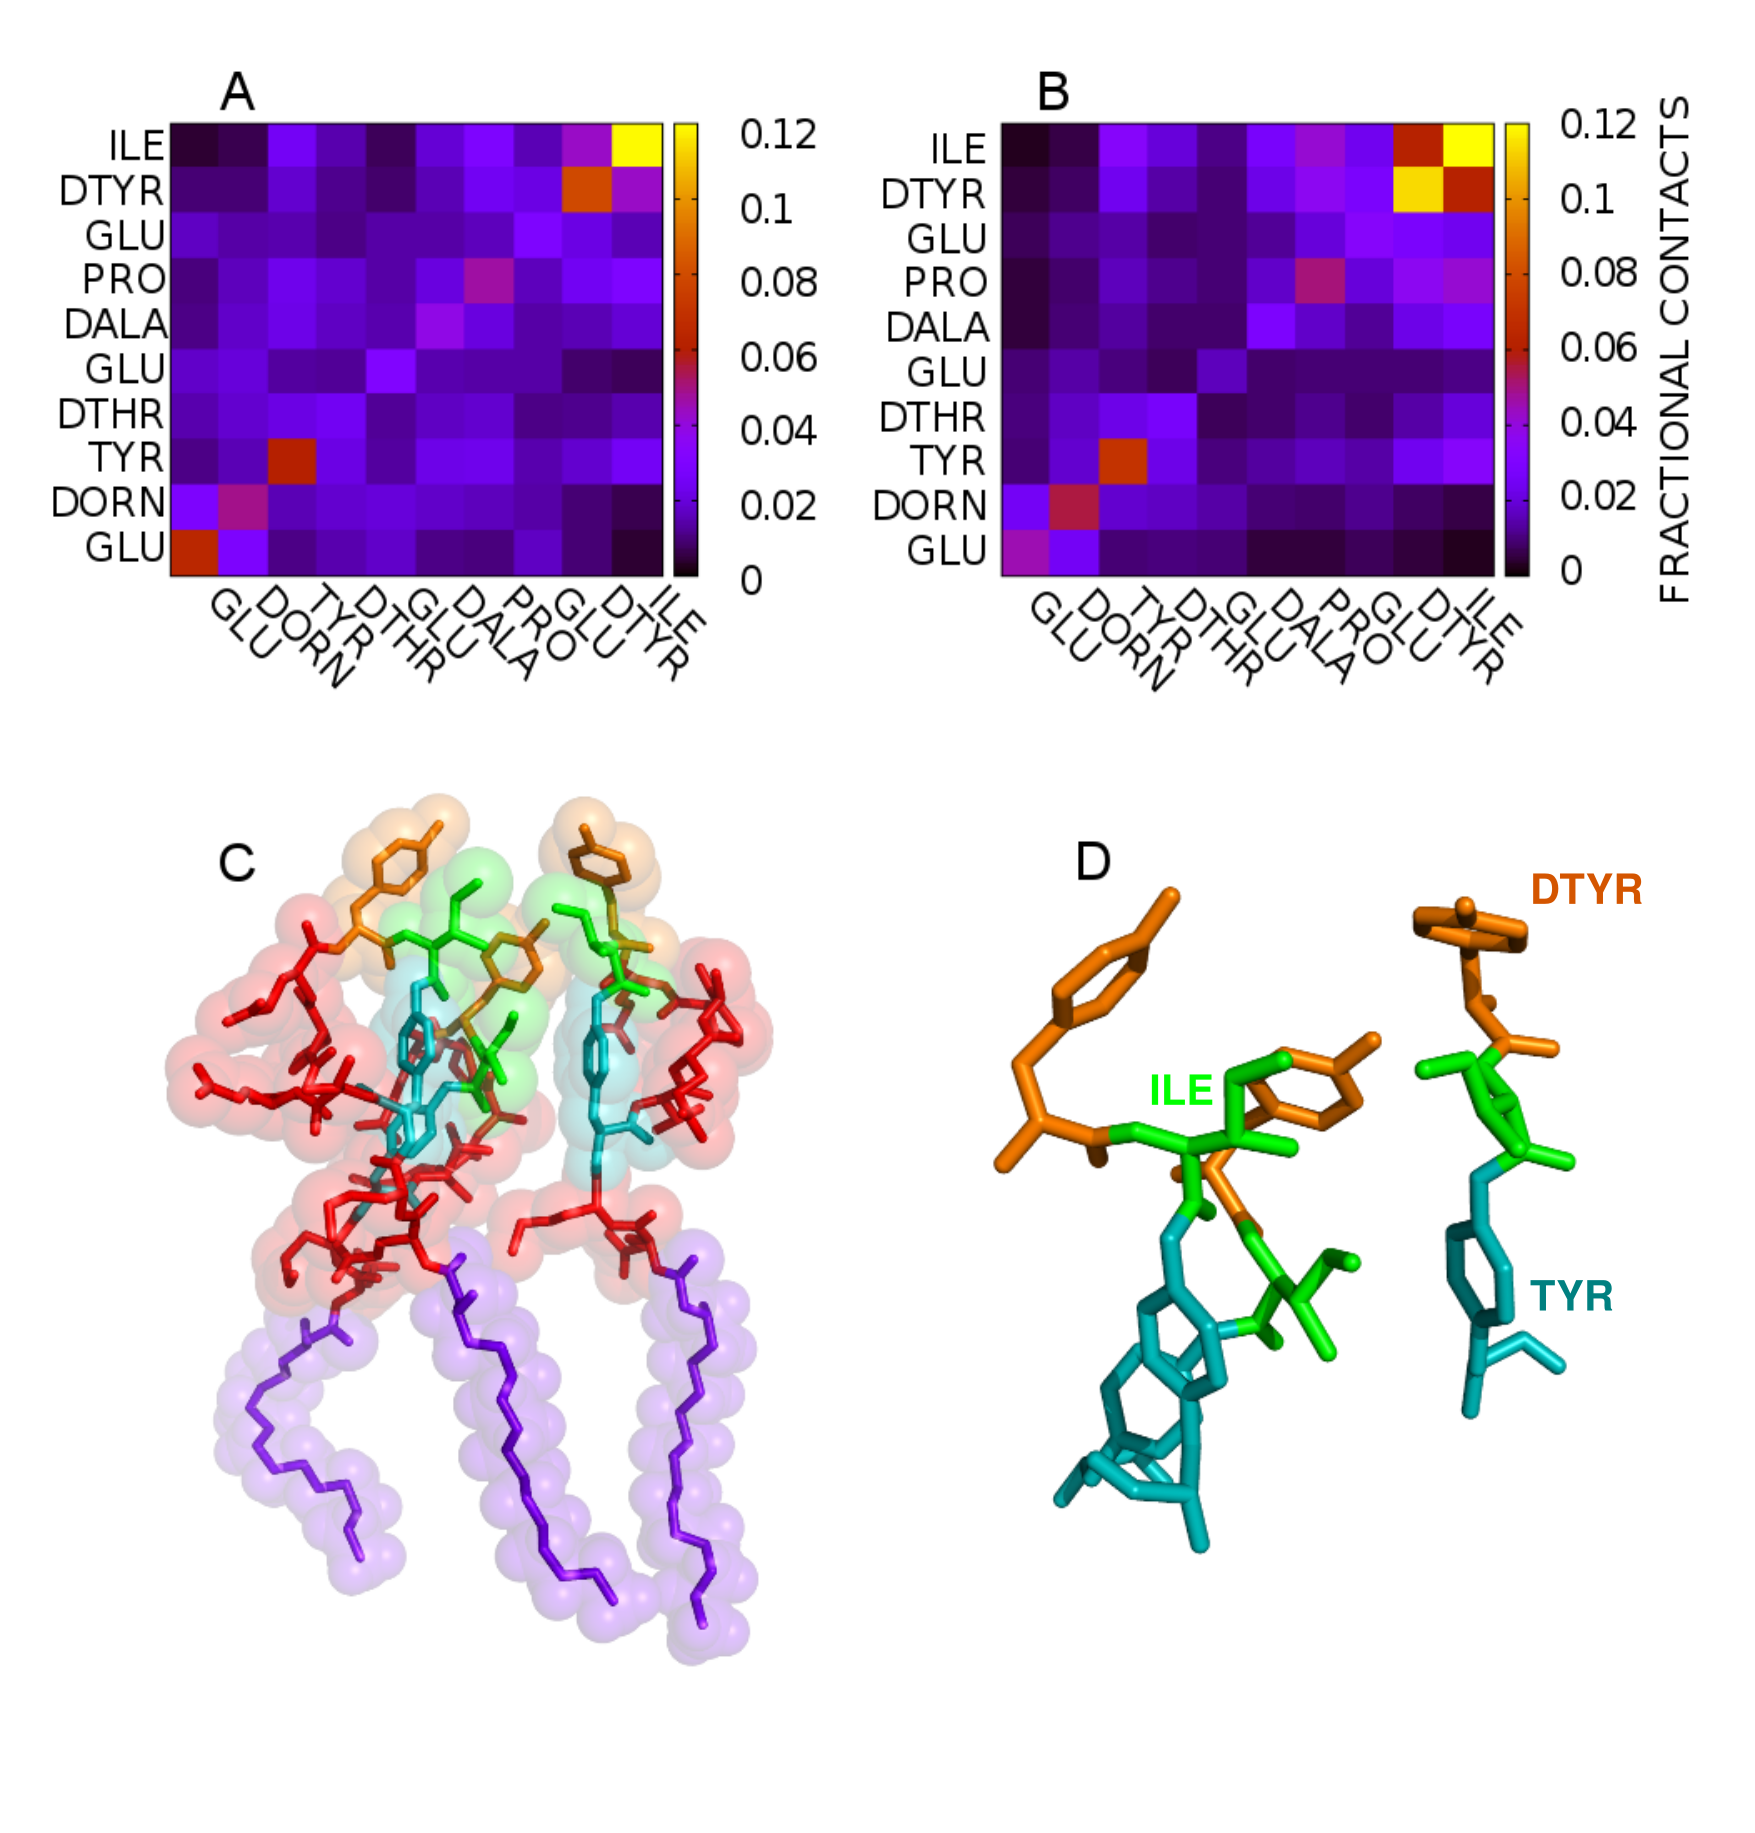
\includegraphics[width=0.7\textwidth]{chapter2_figs/paper_amino_svg.png}
\caption{\label{fig:ch2_amino_contacts}Fractional contacts between fengycin residues which are in contact at (A) PE:PG and (B)PC membranes.
(C) shows three fengycins which are in contact while (D) shows the residues in fengycins that have higher fractional contact value in both
(A) and (B). Yellow, Green and Cyan sticks represents the connectivity in heavy atoms of D-Tyr, Ile and Ring Tyr respectively. Violet
sticks show the acyl tail in fengycin and red represent the peptide bonds.}
\end{figure}

\subsection{Aggregate size is lipid-dependent}
\label{subsec:ch2_aggregate_size}

If the tendency to aggregate is to explain selective targeting of specific
membranes, we should see a difference in the distribution of aggregate sizes
between "bacteria-like" PE:PG membranes and "eukaryotic" PC membranes. Using the
\textbf{\nameref{sss:ch2_agg}} method described in \textbf{\nameref{s:ch2_methods}},  we
calculated the probability distribution  based on aggregate size using fengycins
as the selection shown in \textbf{Figure \ref{fig:ch2_cluster_pop}}. Surprisingly, it looks like
there is a stronger tendency to form larger aggregates (specifically, 7-8mers)
in PE:PG membranes than in PC, in apparent contradiction with \textbf{Figure
\ref{fig:ch2_feng_feng}} which overall indicates a higher probability of
fengycin-fengycin pairs in PC.

This contradiction is resolved by looking at the lifetimes for
different aggregate sizes, plotted in \textbf{Figure \ref{fig:ch2_membrane_lifetime}} (see
section \textbf{\nameref{sss:ch2_lifetime}} in \textbf{\nameref{s:ch2_methods}} for
 discussion of how the lifetimes were computed). \textbf{Figure
\ref{fig:ch2_membrane_lifetime}} shows the autocorrelation curve for
fengycin trimers(3-mers), pentamers(5-mers), and octamers(8-mers) in two different membrane systems, PE:PG and PC.
In PC, trimers have the shortest lifetimes, while
pentamers have longer lifetimes than octamers. By contrast, all three
aggregates sizes have comparable (and very short) lifetimes in PE:PG.
This indicates that small aggregates like trimers are only transient in both membranes,
typically falling apart within 15 ns or so. In PE:PG, the lifetimes have gotten even shorter, with all three aggregates
surviving perhaps 10 ns or so. By contrast, pentamers are longer-lived in PC
membranes, at roughly 100 ns. \textbf{Figure \ref{fig:ch2_membrane_lifetime}A} shows octamers
 are transient structures in PE:PG membranes, but are
metastable in PC as indicated by \textbf{Figure \ref{fig:ch2_membrane_lifetime}B}.
Visual inspection of trajectories clarifies the difference:
when larger aggregates are present in PE:PG, they are nearly always a result of
``collisions'' between smaller aggregates without much in the way of stabilizing
interactions; as a result, they diffuse apart promptly. By contrast, when
larger aggregates form in PC, they are typically stabilized by a combination of
polar interactions near the membrane and hydrophobic ones far from it, as
discussed above. The relative lack of significantly favorable sidechain
interactions with PC headgroups (compared to PE:PG) also likely contributes to
the increased kinetic stability.

\begin{figure}
\centering
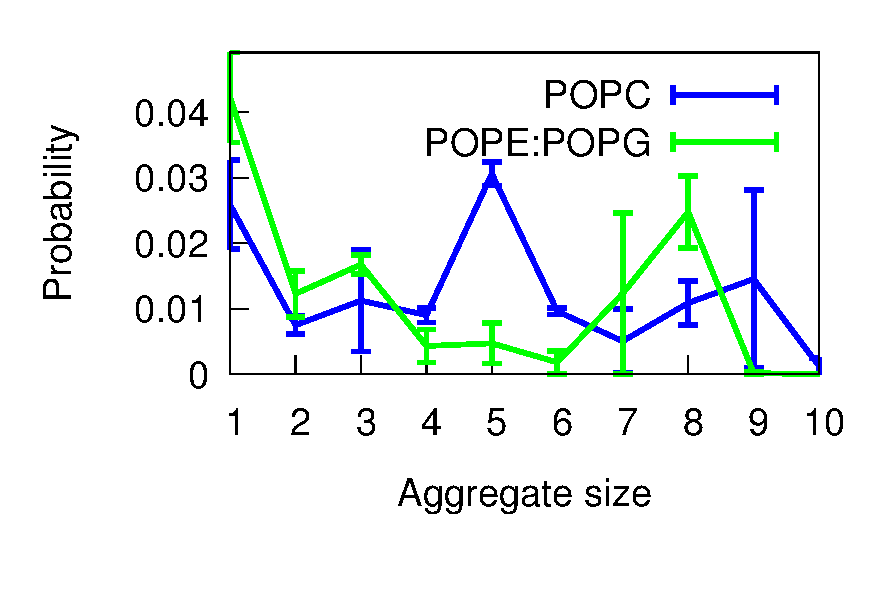
\includegraphics[width=0.4\textwidth]{chapter2_figs/clusters.pdf}
\caption{\label{fig:ch2_cluster_pop} Probability of a specific size fengycin aggregate existing in either of the two membrane systems.}
\end{figure}

\begin{figure}
\centering
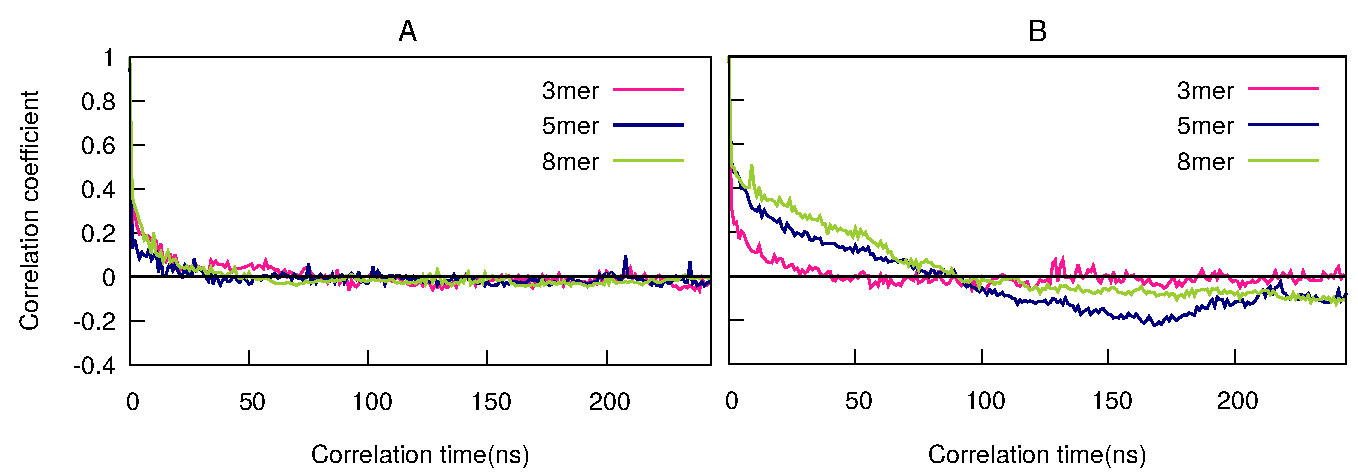
\includegraphics[width=0.8\textwidth]{chapter2_figs/aggs_lipidtype.pdf}
\caption{\label{fig:ch2_membrane_lifetime} Lifetime of 3-mer,5-mer and 8-mer in the two membrane systems (A)PE:PG and (B)PC.
Time delay is along the x-axis while auto-correlation coefficient is along the y-axis.
}
\end{figure}

Going forward, we see several important questions to answer. First, the present
simulations place fengycins on both membrane leaflets, essentially representing
equilibrium conditions accessible in biophysical experiments. However, biologically the
fengycins would ``attack'' from outside the cell, initially binding exclusively to one
leaflet. It is possible that the aggregation differences would be made more
significant by this assymmetry, as suggested by our previous coarse-grained work.\cite{HornGrossfield2013}

Second, it is extremely difficult to quantify the thermodynamics of aggregate
formation on the timescales accessible to all-atom membrane simulations, because
equilibrium simulations would have to run long enough for aggregates to form and
break up multiple times. Quantitatively understanding this thermodynamics \textbf{---}
necessary to test the hypothesis that aggregation controls function \textbf{---} will instead
require some form of enhanced sampling in order to obtain quantitative accuracy.

Finally, we know that fengycins damage fungal membranes, but do far less damage to mammalian membranes, even though both are eukaryotic. Given the interest in using fengycin-like molecules as potential antifungal medicines it would be valuable to understand why they target one organism but not the other.\cite{Rinaldi2009} One likely hypothesis would be to attribute the differences to the sterol present in the fungal vs. mammalian membranes (ergosterol and cholesterol respectively). Some experiments indicate that cholesterol's tendency to increase membrane order may protect mammalian membranes, but the mechanisms are unclear and could likely be revealed by future simulations.\cite{Heerklotz2015}
Similarly, the presence of different anionic lipids in fungal membranes (e.g. phosphatidylinositol) may also play a role, particularly if their behavior is different from anionic lipids found in bacteria such as PG.
\newpage

\section{Conclusions}
\label{s:conclu}

Fengycins operate as biological fungicides primarily by targeting and damaging
the fungus' outer membranes, while leaving their plant hosts and the bacteria
that produce them unharmed.  We used all-atom molecular dynamics simulations of
fengycin molecules bound to two membrane compositions (PE:PG and PC) chosen as
simple mimics of bacterial and eukaryotic membranes in order to explain this
functional selectivity. In particular, we showed that while fengycin binding
disorders the lipid hydrophobic region independent of headgroup type, its
aggregation propensities varies with lipid composition. Although aggregates form
in both membrane types, larger aggregates are only stable in the eukaryotic-like
membranes representative of their target fungi.

In  addition, fengycin perturbs the membrane irrespective of the lipid composition,
but the extent of membrane leakage is traced back to formation of aggregates.
Hence the aggregation process itself depends on the tug of war between two favoring interactions.
One is the hydrophobic interactions between Tyr-10, Tyr-4 and Ile-11 of adjacent fengycins
which lead to stable aggregates and the other is the favorable electrostatic interactions between
fengycin's charged residues (glutamates and ornithine) and the lipid head groups. These two attractive
 and repulsive forces determine whether fengycin will form aggregates on membrane surfaces or not
and thus regulate the membrane selectivity of fengycin.

